\documentclass[a2paper, 12pt]{article}
\usepackage[font={huge, bf}]{caption}
\usepackage{fontspec}
\setmainfont{Arial}
\usepackage{subcaption}
\usepackage{graphicx}
\usepackage{tikz}
\usepackage{tikzsymbols}
\usetikzlibrary{calc,patterns,shapes.geometric}
\usepackage{float}
\usepackage{pdflscape}
\usepackage{geometry}
\geometry{landscape, margin=2cm}
\captionsetup[subfigure]{justification=justified,singlelinecheck=false}
\pagestyle{empty}

\def\centerarc[#1](#2)(#3:#4:#5){\draw[#1] ($(#2)+({#5*cos(#3)},{#5*sin(#3)})$) arc (#3:#4:#5);}

\begin{document}
	\vspace*{\fill}
	\begin{figure}[!htbp]
		\centering
		\begin{subfigure}[b]{0.48\textwidth}
			\caption{Figure 1}
			\centering
			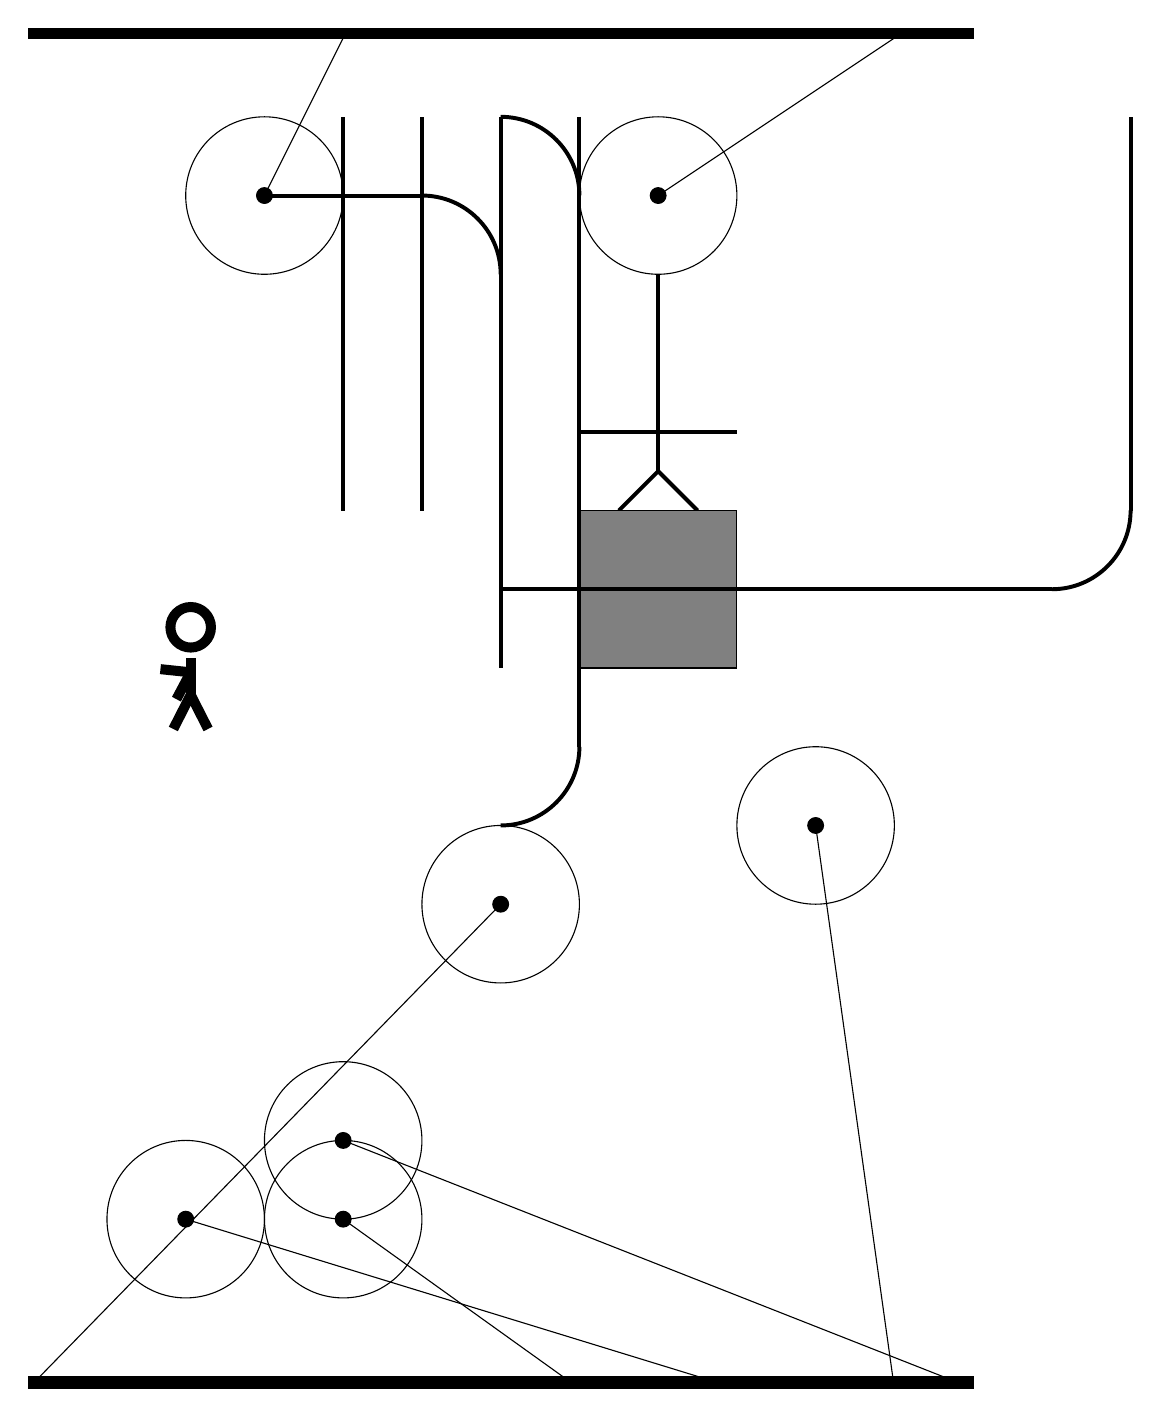
\begin{tikzpicture}
				\draw[fill=black] (-2, 14) rectangle (10, 14.125);
				
				\draw (1,12) circle (1);
				\draw[fill=black] (1,12) circle (0.1);
				\draw (2,14.0) -- (1,12);
				
				\draw (2,-1) circle (1);
				\draw[fill=black] (2,-1) circle (0.1);
				\draw (5,-3.15) -- (2,-1);
				
				\draw (0,-1) circle (1);
				\draw[fill=black] (0,-1) circle (0.1);
				\draw (7,-3.15) -- (0,-1);
				
				\draw (4,3) circle (1);
				\draw[fill=black] (4,3) circle (0.1);
				\draw (-2,-3.15) -- (4,3);
				
				\draw (2,0) circle (1);
				\draw[fill=black] (2,0) circle (0.1);
				\draw (10,-3.15) -- (2,0);
				
				\draw (8,4) circle (1);
				\draw[fill=black] (8,4) circle (0.1);
				\draw (9,-3.15) -- (8,4);
				
				\draw (6,12) circle (1);
				\draw[fill=black] (6,12) circle (0.1);
				\draw (9,14.0) -- (6,12);
				
				\draw[line width=0.5mm](6,8.5) -- (6,11.0);
				\draw[line width=0.5mm](5.5,8) --  (6,8.5) -- (6.5,8);
				\draw[fill=black!50] (5, 8) rectangle (7, 6);
				
				\draw[line width = 0.5mm] (4,7) -- (11,7);
				\draw[line width = 0.5mm] (11,7) arc (270:360:1);
				\draw[line width = 0.5mm] (12,8) -- (12,13);
				\draw[line width = 0.5mm] (3,8) -- (3,13);
				\centerarc[line width = 0.5mm](4,13)(0:180:1);
				\draw[line width = 0.5mm] (5,13) -- (5,10);
				\centerarc[line width = 0.5mm](6,10)(270:180:1);
				\draw[line width = 0.5mm] (6,9) -- (7,9);
				\draw[line width = 0.5mm] (4,4) arc (270:360:1);
				\draw[line width = 0.5mm] (5,5) -- (5,12);
				\draw[line width = 0.5mm] (5,12) arc (0:90:1);
				\draw[line width = 0.5mm] (4,6) -- (4,11);
				\draw[line width = 0.5mm] (3,12) arc (90:0:1);
				\draw[line width = 0.5mm] (3,12) -- (1,12);
				\draw[line width = 0.5mm] (2,8) -- (2,13);
				\centerarc[line width = 0.5mm](3,13)(0:180:1);
				\draw[line width = 0.5mm] (4,13) -- (4,10);
				\centerarc[line width = 0.5mm](5,10)(270:180:1);
				\draw[line width = 0.5mm] (5,9) -- (6,9);
				
				\node at (0, 6) {\scriptsize \Strichmaxerl[10][62][174]};
				
				\draw[fill=black] (-2, -3) rectangle (10, -3.15);
			\end{tikzpicture}
		\end{subfigure}
		\hfill
		\begin{subfigure}[b]{0.48\textwidth}
			\caption{Figure 2}
			\centering
			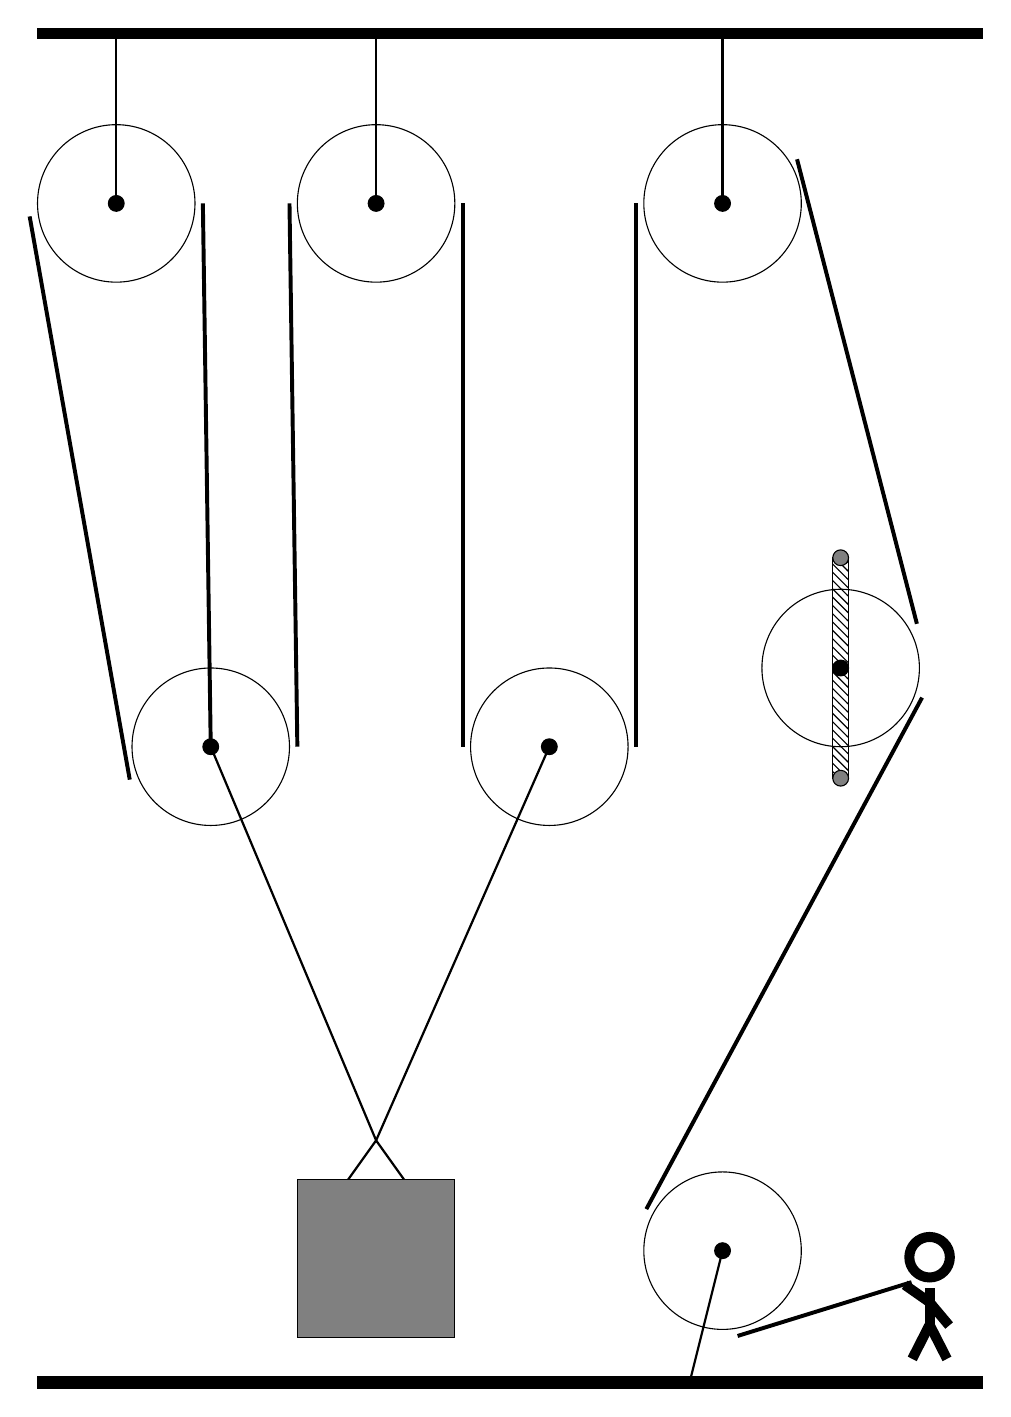
\begin{tikzpicture}
				\draw[fill=black] (-2, 14) rectangle (10, 14.125);
				
				\draw (-1, 11.9) circle (1);
				\draw[fill=black] (-1, 11.9) circle (0.1);
				\draw[thick] (-1, 11.9) -- (-1, 14);
				
				\draw (2.3, 11.9) circle (1);
				\draw[fill=black] (2.3, 11.9) circle (0.1);
				\draw[thick] (2.3, 11.9) -- (2.3, 14);
				
				\draw (6.7, 11.9) circle (1);
				\draw[fill=black] (6.7, 11.9) circle (0.1);
				\draw[thick] (6.7, 11.9) -- (6.7, 14);
				
				\draw (0.2, 5) circle (1);
				\draw[fill=black] (0.2, 5) circle (0.1);
				
				\draw (4.5, 5) circle (1);
				\draw[fill=black] (4.5, 5) circle (0.1);
				
				\draw (8.2, 6) circle (1);
				\draw[fill=black] (8.2, 6) circle (0.1);
				\draw[pattern=north west lines, pattern color=black] (8.1, 7.4) rectangle (8.3, 4.6);
				\draw[fill=black!50] (8.2, 7.4) circle (0.1);
				\draw[fill=black!50] (8.2, 4.6) circle (0.1);
				
				\draw (6.7, -1.4) circle (1);
				\draw[fill=black] (6.7, -1.4) circle (0.1);
				\draw[thick] (6.7, -1.4) -- (6.3, -3);
				
				\draw[thick] (0.2, 5) -- (2.3, 0)  -- (4.5, 5);
				\draw[thick]  (1.8, -0.7) -- (2.3, 0) -- (2.8, -0.7);
				\draw[fill=black!50] (1.3, -0.5) rectangle (3.3, -2.5);
				\draw[line width=0.5mm] (0.2, 5) -- (0.1, 11.9);
				\centerarc[line width=0.5mm](-1, 11.9)(0:200:1.1);
				\draw[line width=0.5mm] (-2.1, 11.735) -- (-0.8285, 4.582);
				\centerarc[line width=0.5mm](0.2, 5)(200:360:1.1);
				\draw[line width=0.5mm](1.3, 5) -- (1.2, 11.9);
				\centerarc[line width=0.5mm](2.3, 11.9)(0:180:1.1);
				\draw[line width=0.5mm] (3.4, 11.9) -- (3.4, 5);
				\centerarc[line width=0.5mm](4.5, 5)(180:360:1.1);
				\draw[line width=0.5mm] (5.6, 5) -- (5.6, 11.9);
				\centerarc[line width=0.5mm](6.7, 11.9)(30:180:1.1);
				\draw[line width=0.5mm](7.646, 12.461) -- (9.168, 6.561);
				\centerarc[line width=0.5mm](8.2, 6)(160:211:-1.1);
				\draw[line width=0.5mm](9.2337, 5.6238) -- (5.732, -0.872);
				\centerarc[line width=0.5mm](6.7, -1.4)(150:280:1.1);
				\draw[line width=0.5mm](6.891, -2.4833) -- (9.1, -1.8);
				
				\node at (9.3, -2) {\scriptsize \Strichmaxerl[10][-35][-50]};
				
				\draw[fill=black] (-2, -3) rectangle (10, -3.15);
			\end{tikzpicture}
		\end{subfigure}
	\end{figure}
		\vspace*{\fill}
\end{document}